\begin{frame}{Antecedentes}

\begin{figure}[h]
	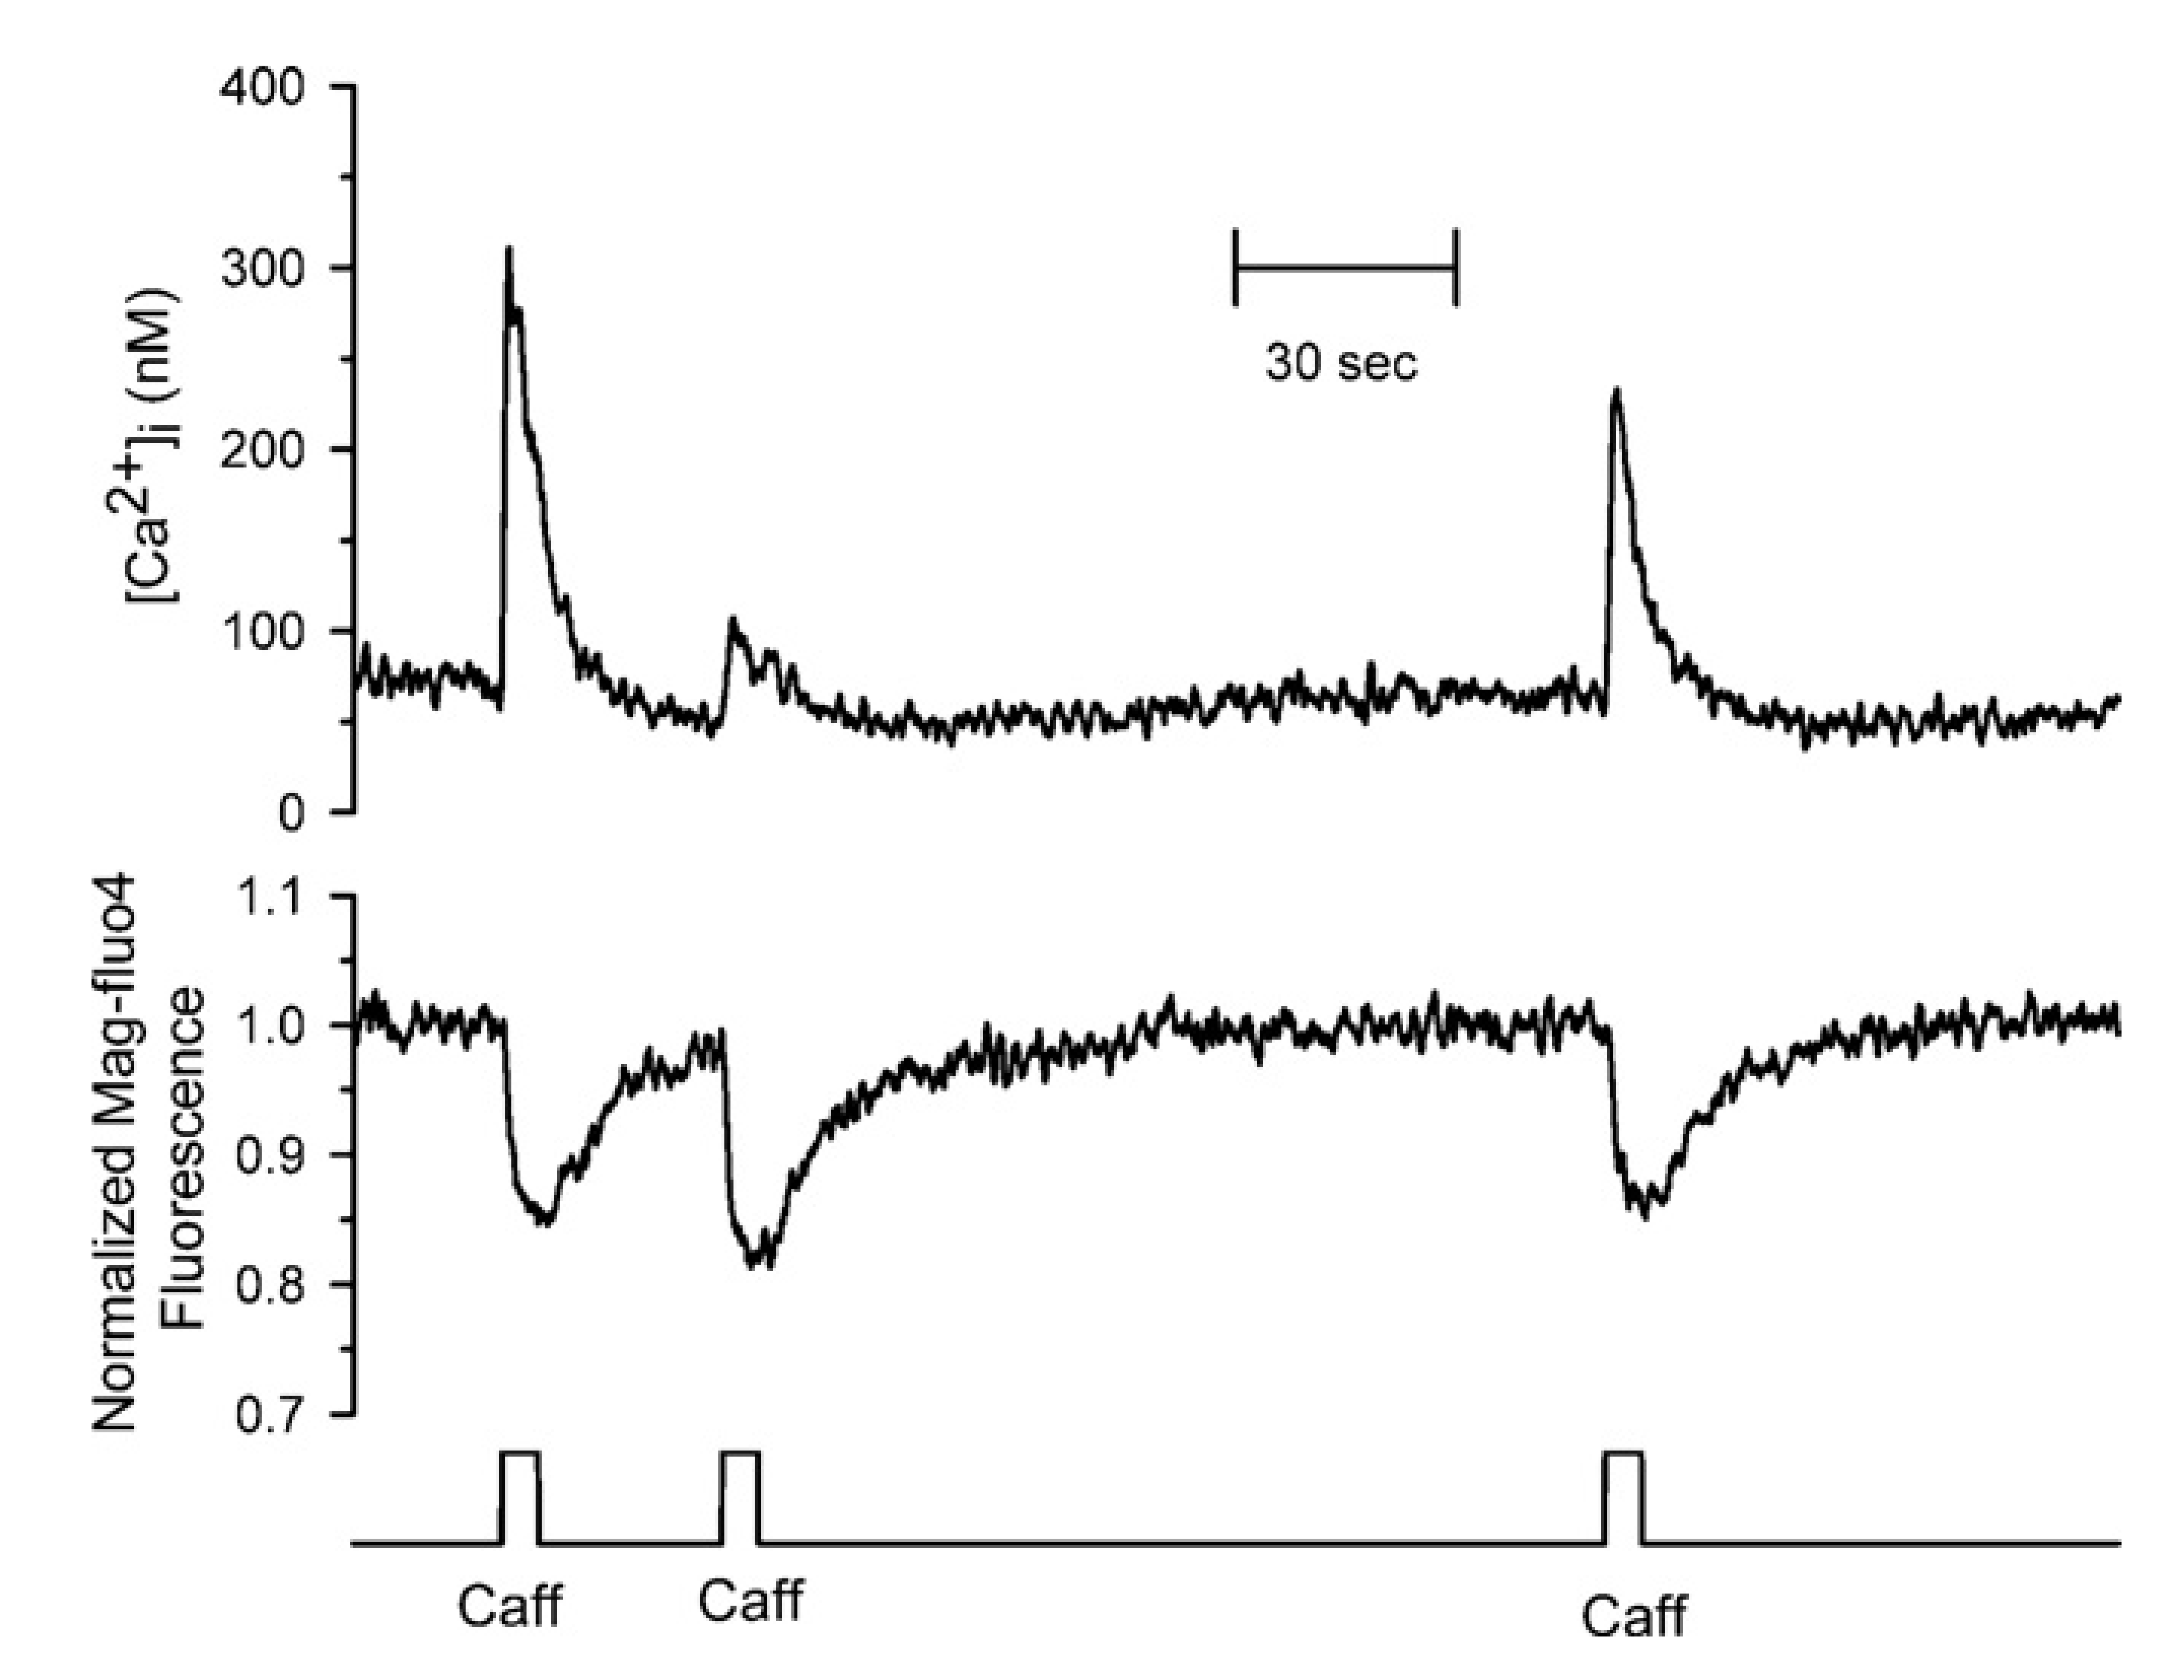
\includegraphics{FIGURA1}
	\caption{{\tiny Adán Dagnino-Acosta and Agustín Guerrero-Hernández. Variable luminal sarcoplasmic
		reticulum Ca2+ buffer capacity in smooth muscle cells. Cell Calcium, 46(3):188–196, sep 2009.}}
\end{figure}

\end{frame}

\begin{frame}{Antecedentes}
	
	\begin{figure}[h]
		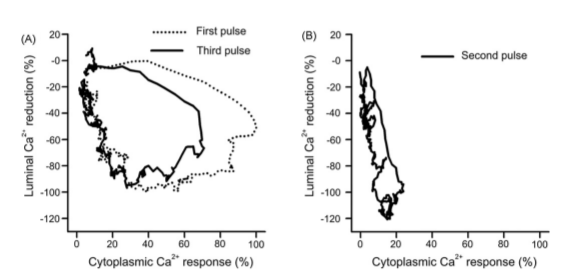
\includegraphics[width=\textwidth]{FIGURA3}
		\caption{{\tiny Agustin Guerrero-Hernandez, Adan Dagnino-Acosta, and Alexei Verkhratsky. An intelligent sarco-endoplasmic reticulum Ca2+ store: Release and leak channels have differential access to a concealed Ca2+ pool. Cell Calcium, 48(2):143–149, 2010.}}
	\end{figure}
	
\end{frame}

\begin{frame}{Antecedentes}
	
	\begin{figure}[h]
		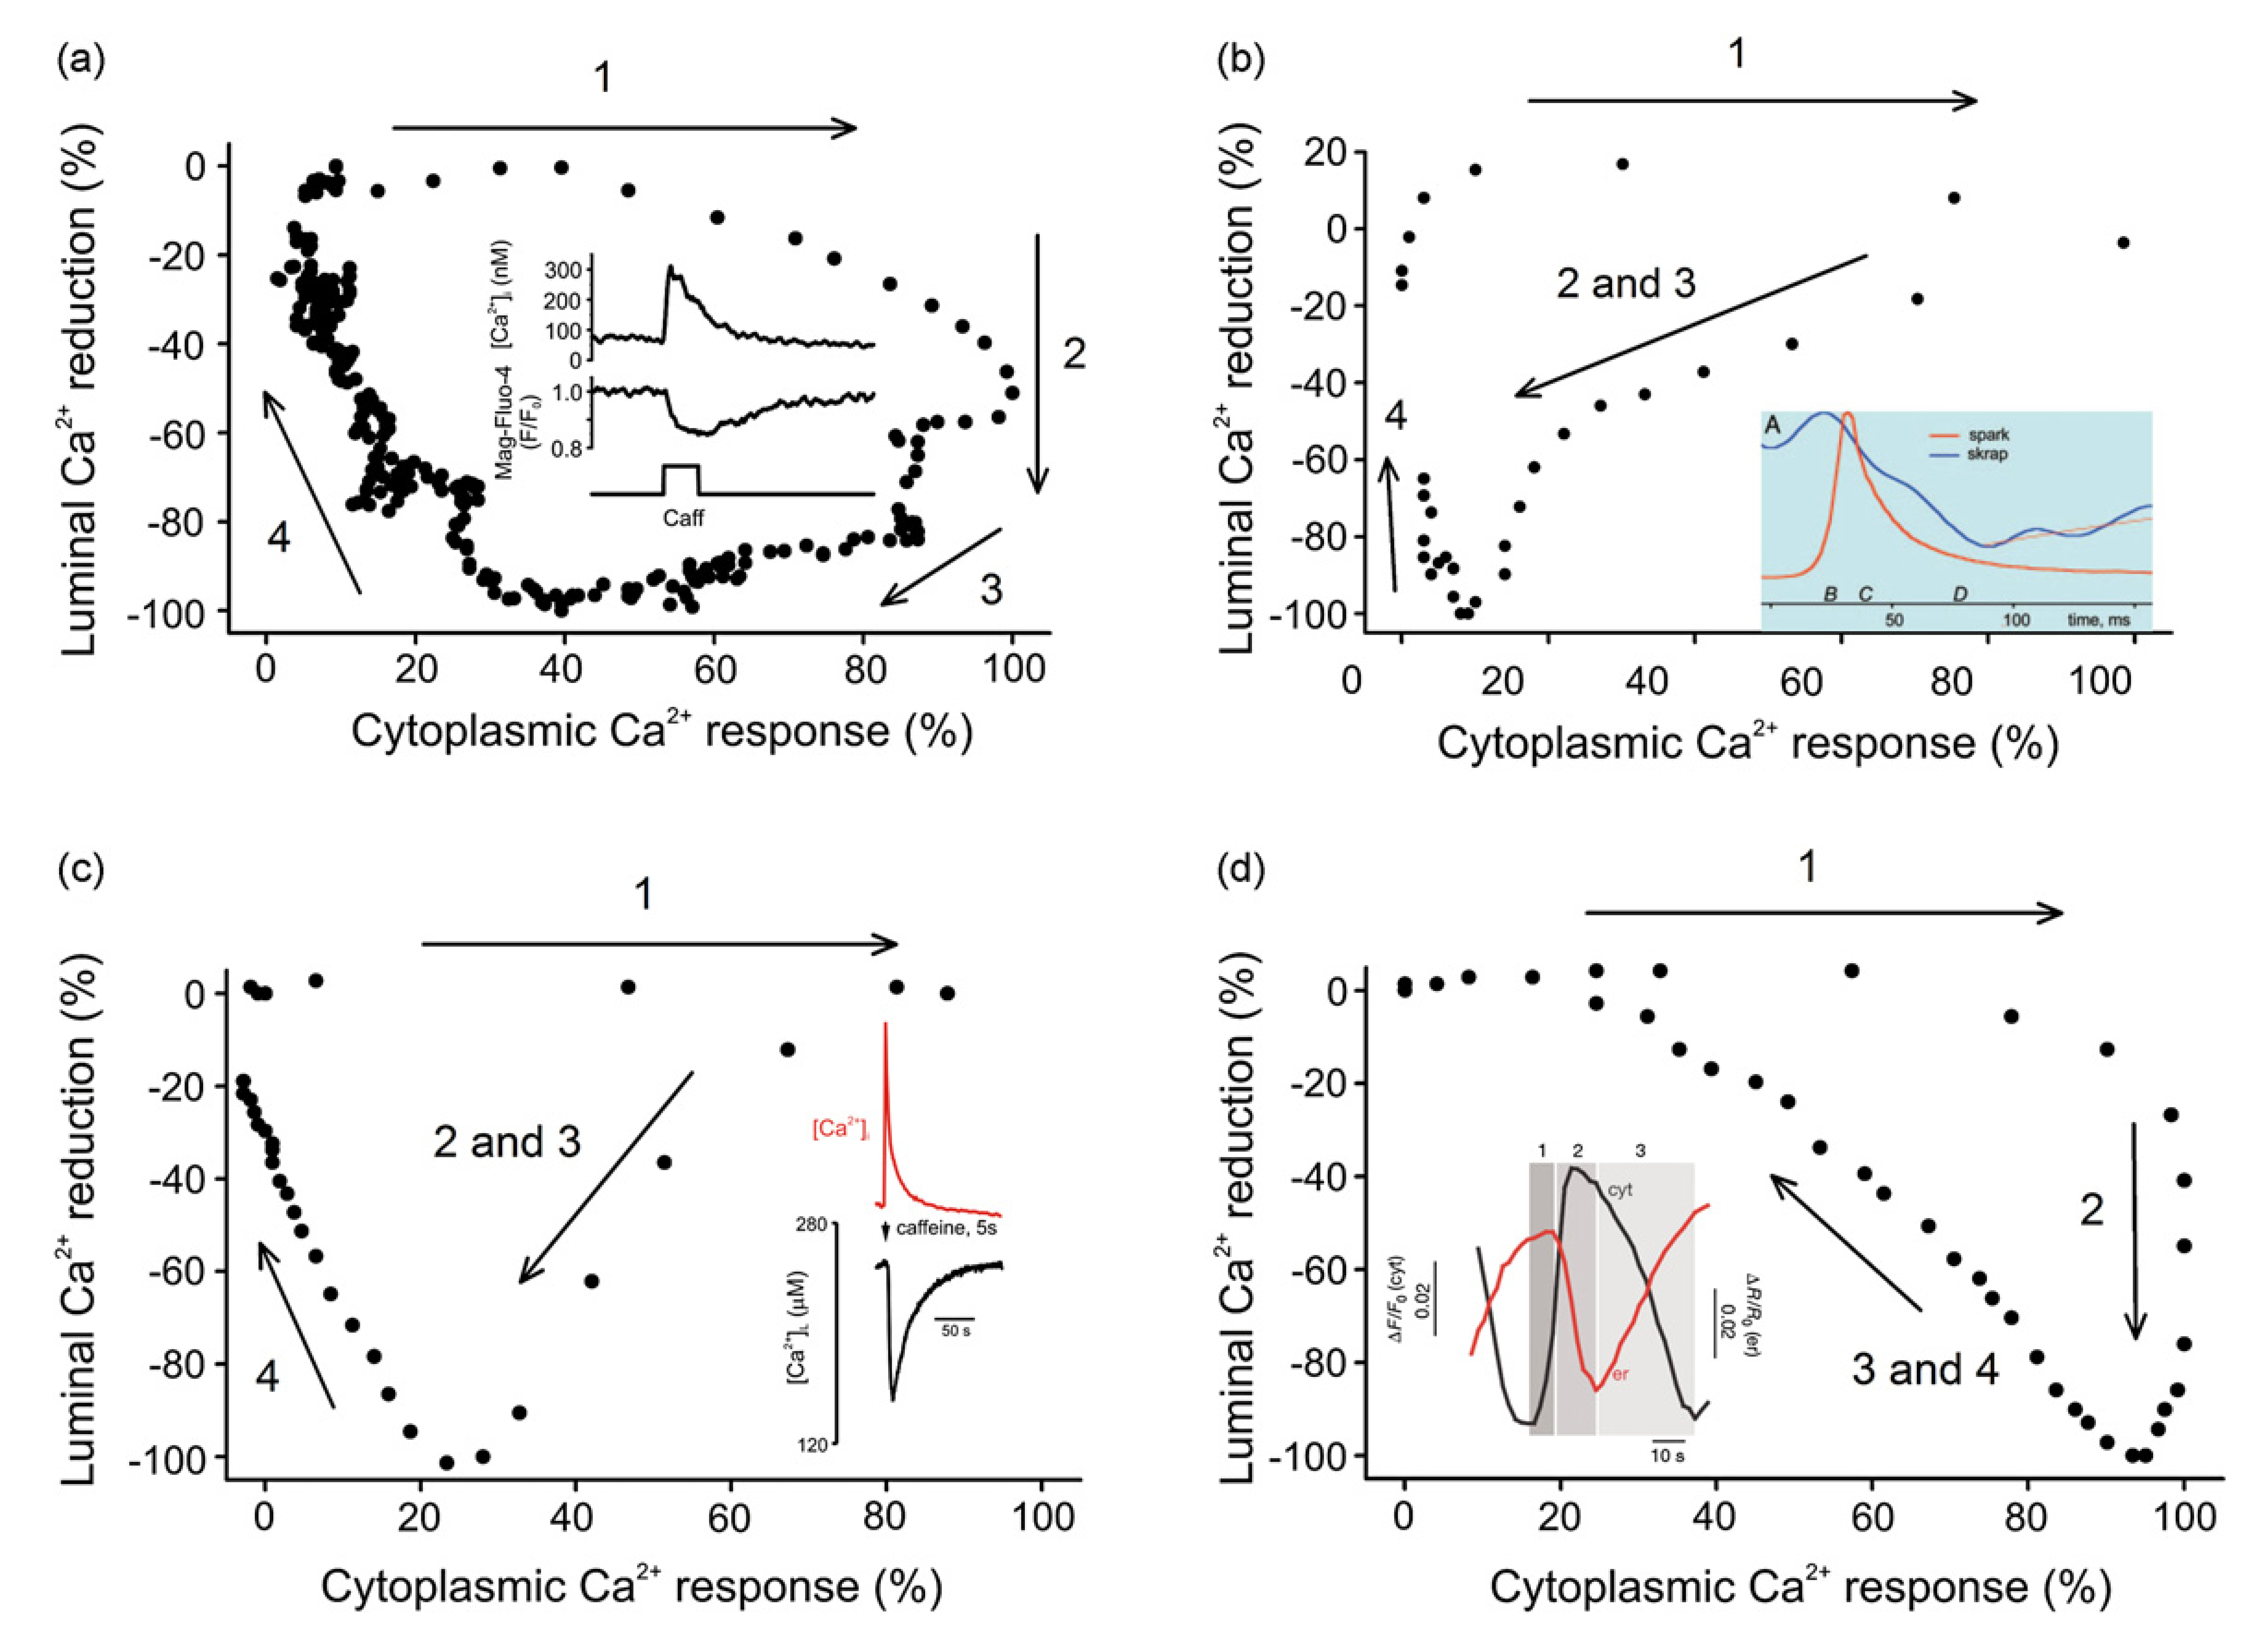
\includegraphics[width=.9\textwidth]{FIGURA2}
		\caption{{\tiny Agustin Guerrero-Hernandez, Adan Dagnino-Acosta, and Alexei Verkhratsky. An intelligent
				sarco-endoplasmic reticulum Ca2+ store: Release and leak channels have differential access
				to a concealed Ca2+ pool. Cell Calcium, 48(2):143–149, 2010.}}
	\end{figure}
	
\end{frame}

\begin{frame}{Antecedentes}
	
	\begin{figure}[h]
		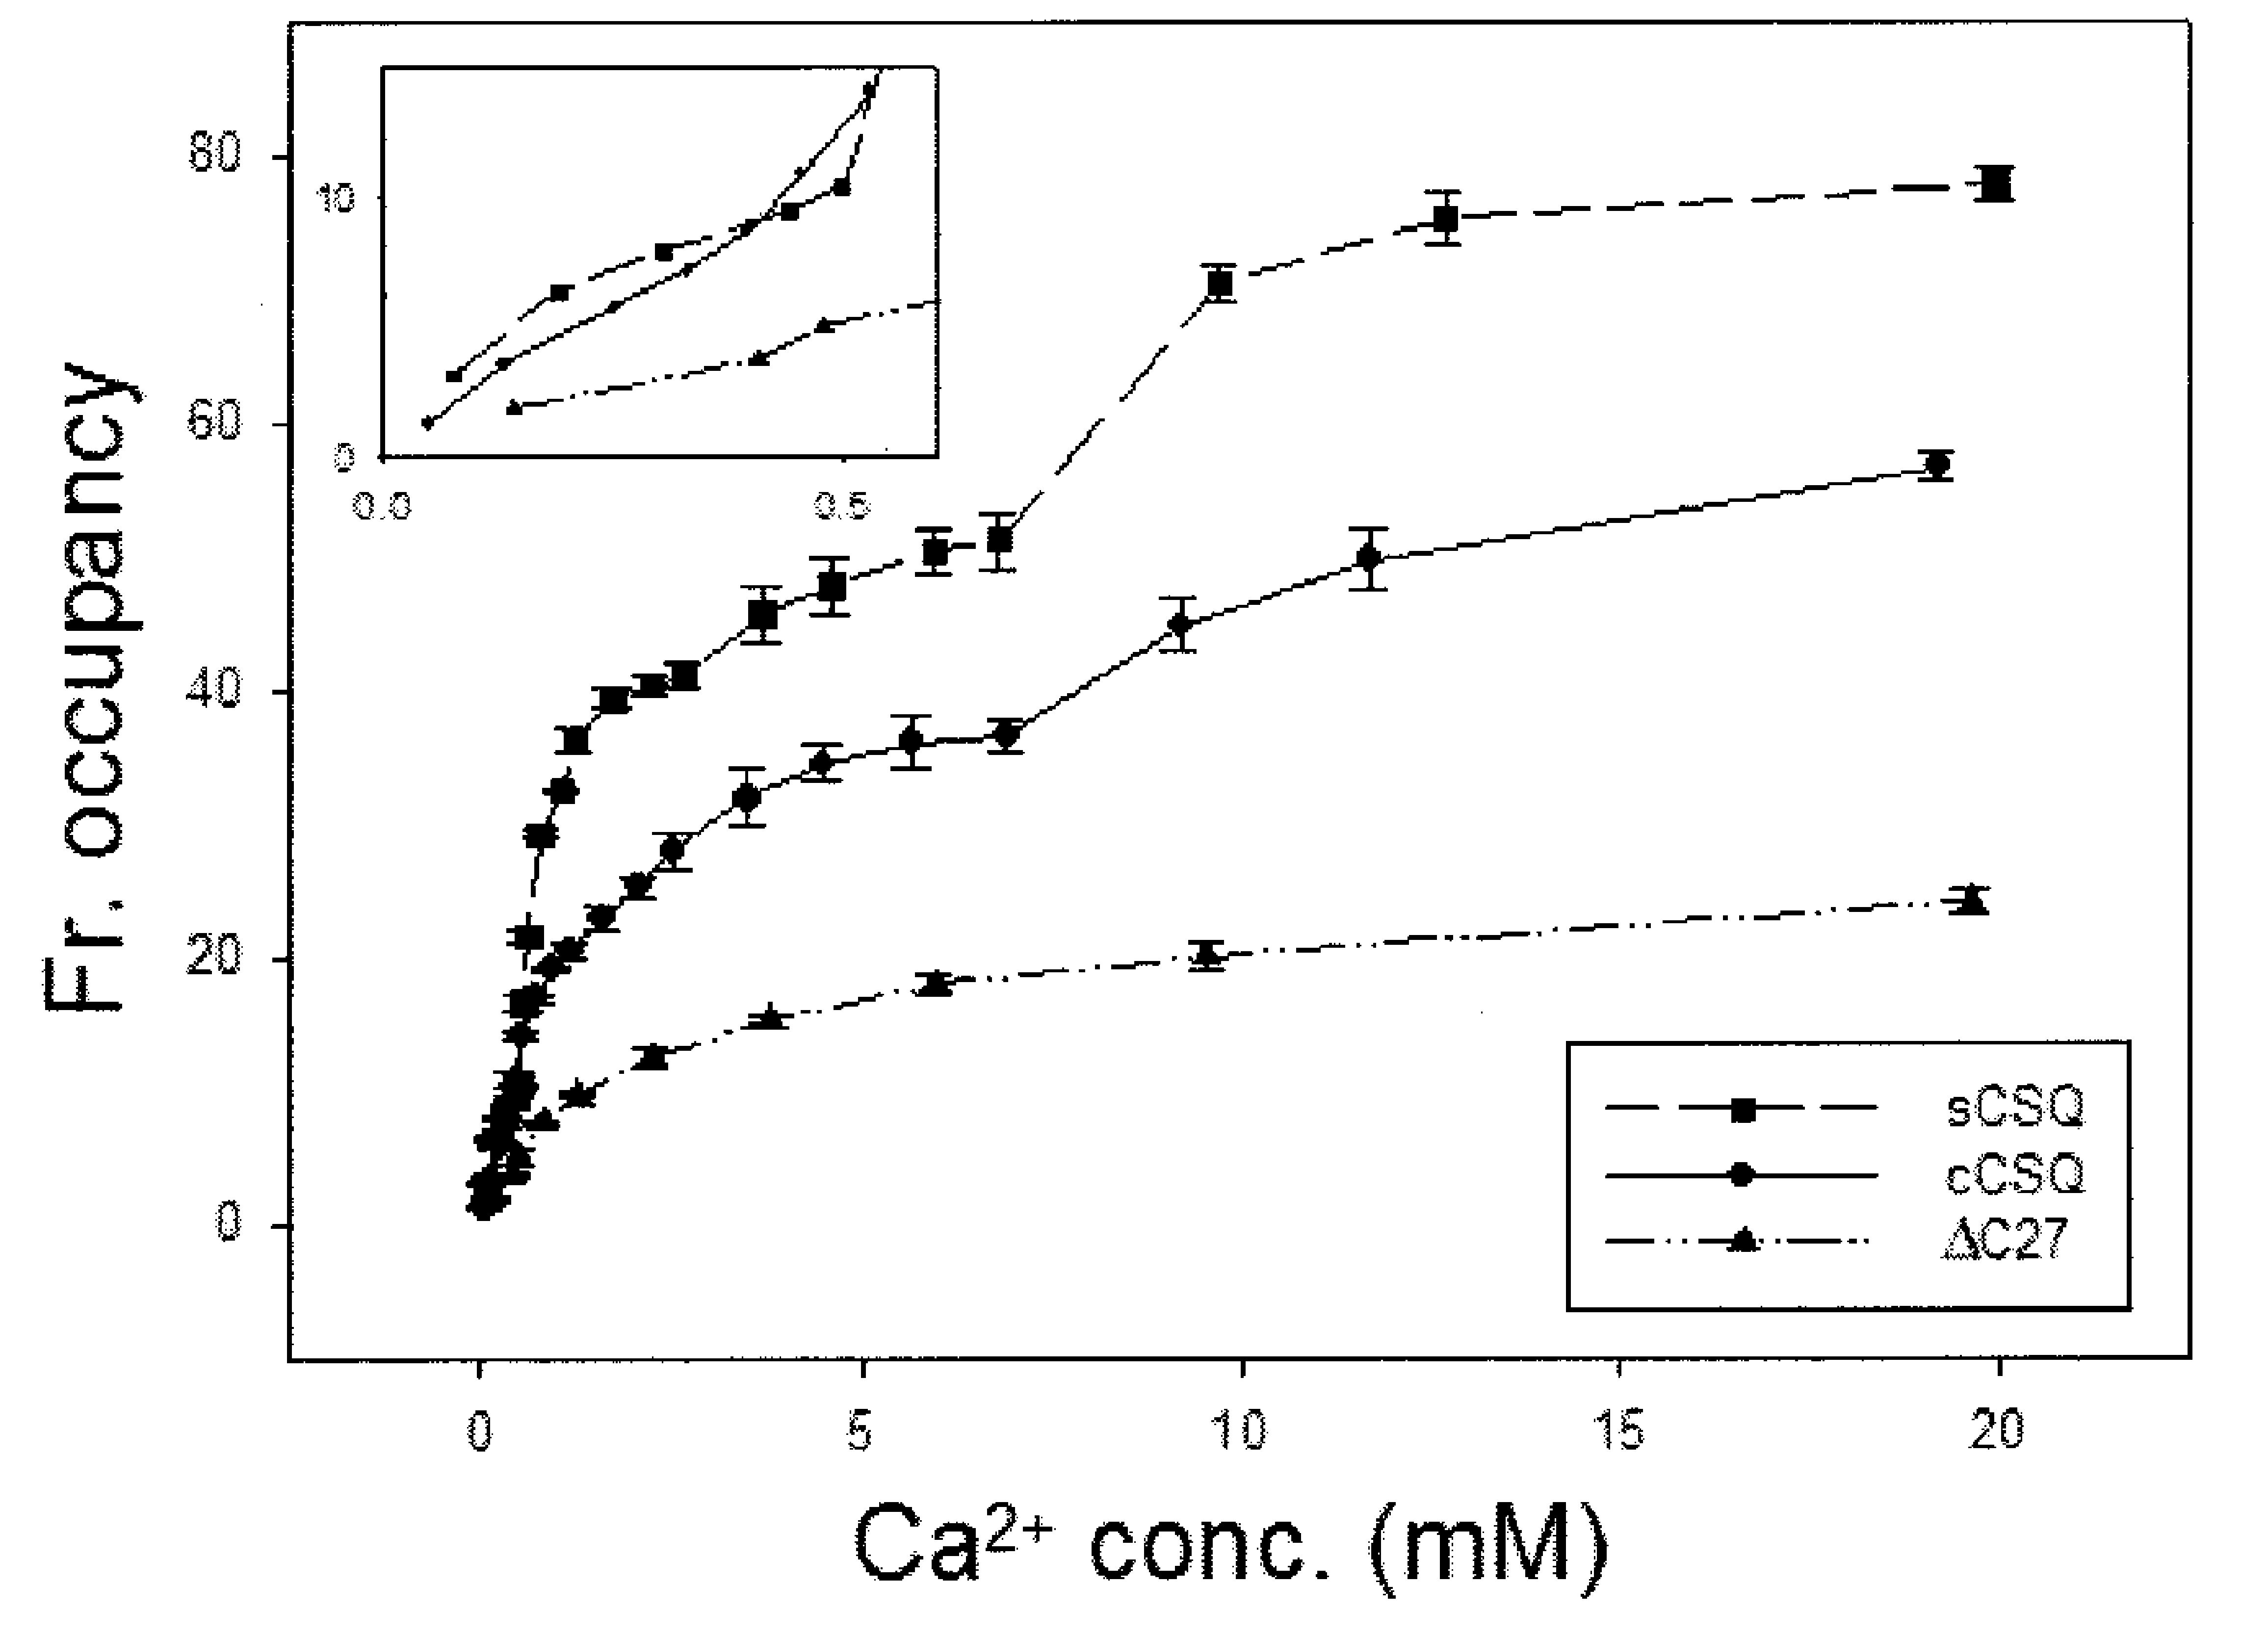
\includegraphics[width=.8\textwidth]{FIGURA9}
		\caption{{\tiny HaJeung Park, Yeong Il Park, EunJung Kim, Buhyun Youn, Kelly Fields, A. Keith Dunker, and
				ChulHee Kang. Comparing skeletal and cardiac calsequestrin structures and their calcium
				binding: A proposed mechanism for coupled calcium binding and protein polymerization.
				Journal of Biological Chemistry, 279(17):18026–18033, 2004.}}
	\end{figure}
	
\end{frame}

\begin{frame}{Antecedentes}
	
	\begin{figure}[h]
		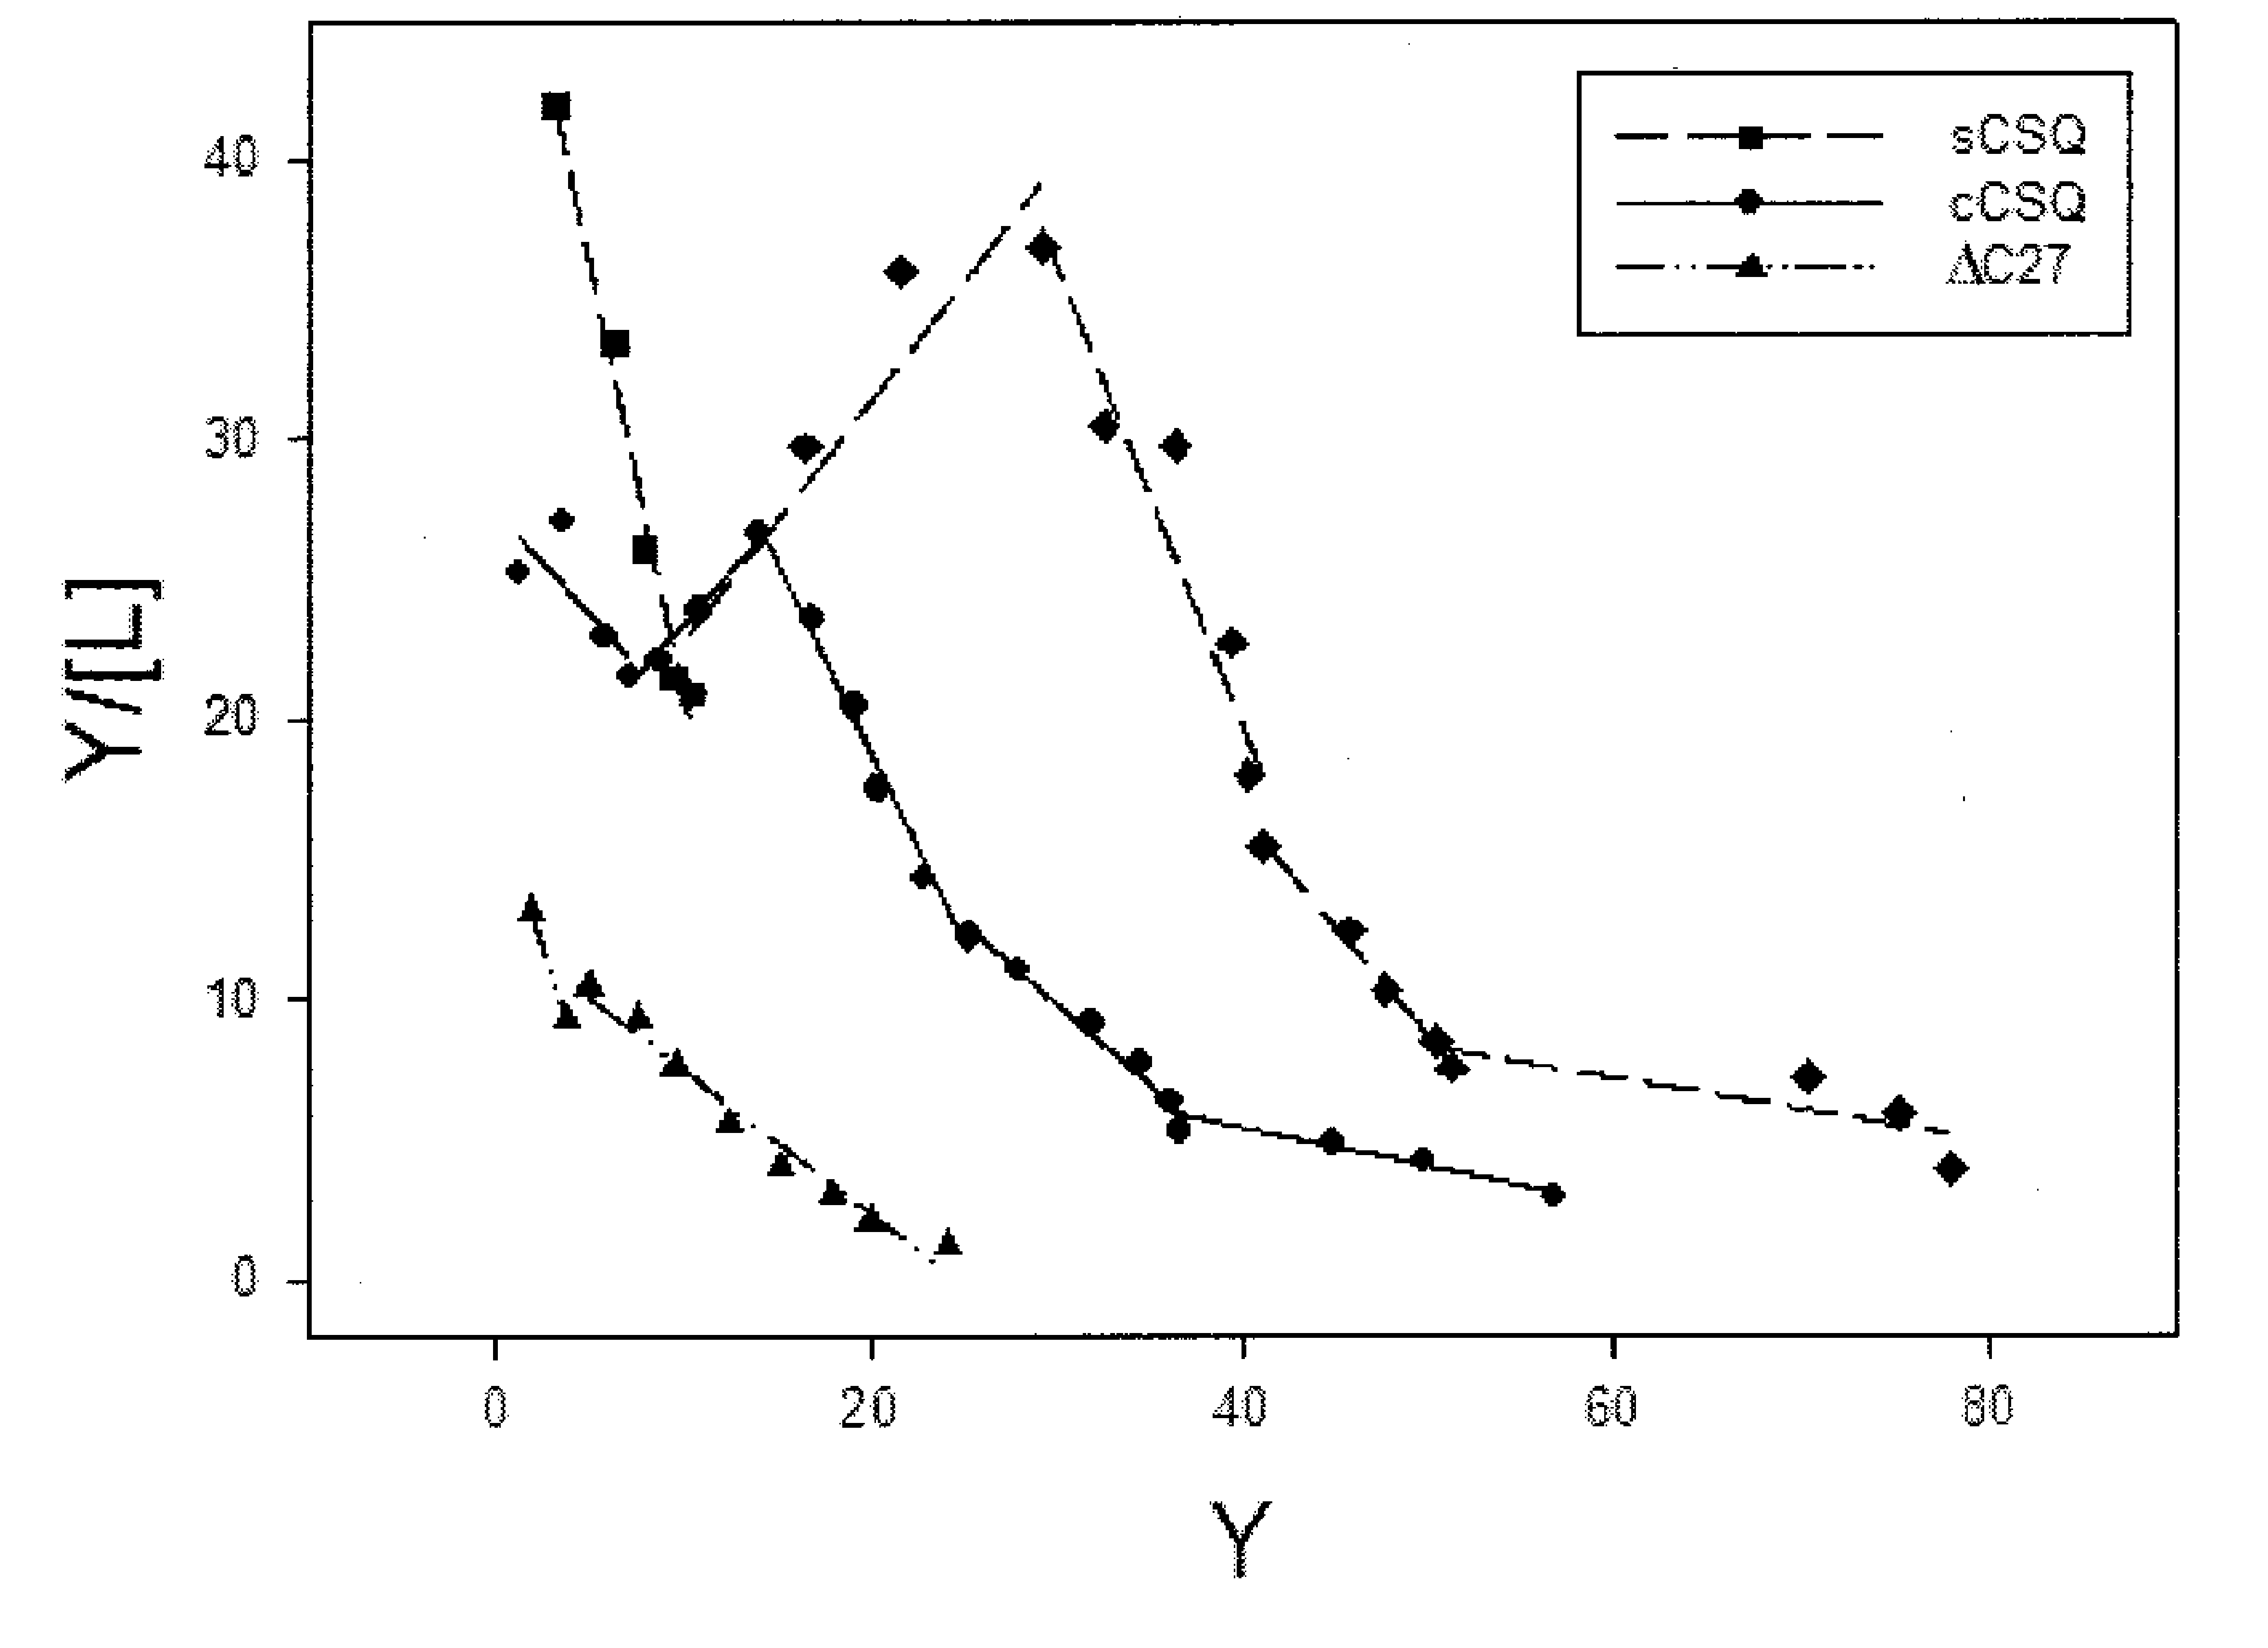
\includegraphics[width=.8\textwidth]{FIGURA10}
		\caption{{\tiny HaJeung Park, Yeong Il Park, EunJung Kim, Buhyun Youn, Kelly Fields, A. Keith Dunker, and
				ChulHee Kang. Comparing skeletal and cardiac calsequestrin structures and their calcium
				binding: A proposed mechanism for coupled calcium binding and protein polymerization.
				Journal of Biological Chemistry, 279(17):18026–18033, 2004.}}
	\end{figure}
	
\end{frame}

\begin{frame}{Antecedentes}
	
	\begin{figure}[h]
		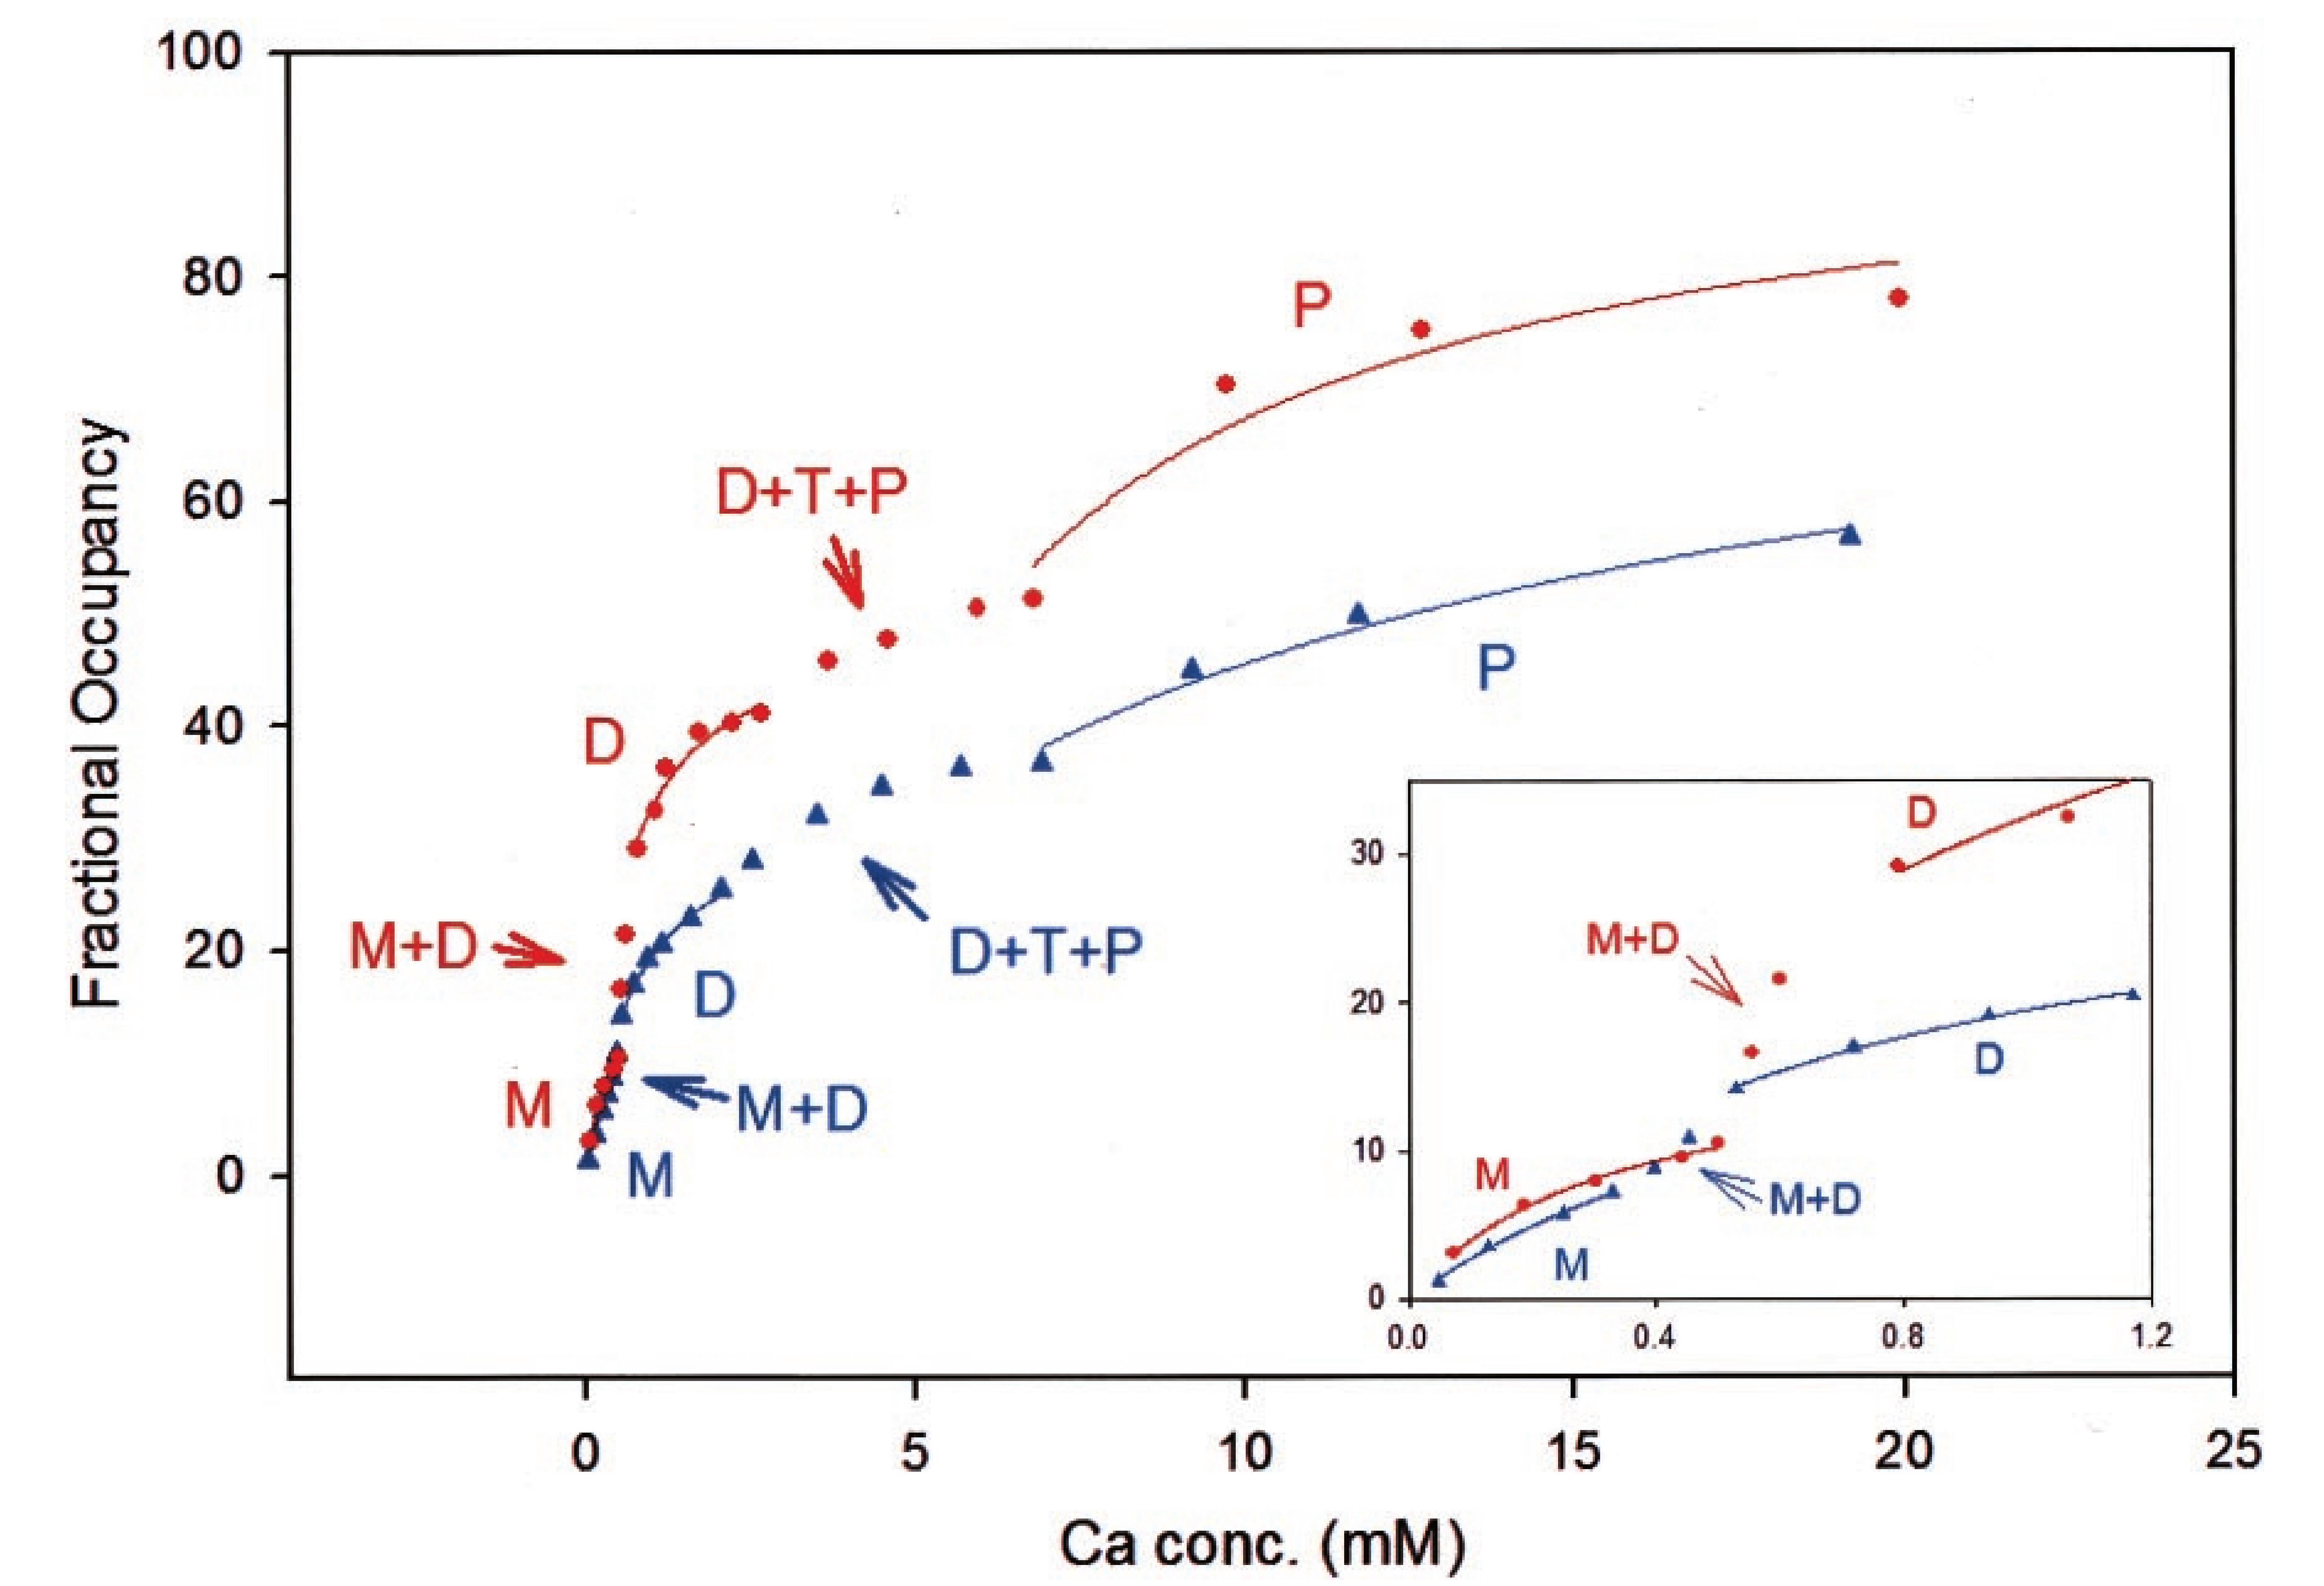
\includegraphics[width=.8\textwidth]{FIGURA11}
		\caption{{\tiny HaJeung Park, Yeong Il Park, EunJung Kim, Buhyun Youn, Kelly Fields, A. Keith Dunker, and
				ChulHee Kang. Comparing skeletal and cardiac calsequestrin structures and their calcium
				binding: A proposed mechanism for coupled calcium binding and protein polymerization.
				Journal of Biological Chemistry, 279(17):18026–18033, 2004.}}
	\end{figure}
	
\end{frame}

\begin{frame}{Antecedentes}
	
	\begin{figure}[h]
		\includegraphics[width=.7\textwidth]{FIGURA4}
		\caption{{\tiny Norma C. Perez-Rosas, Norma L. Gomez-Viquez, Adan Dagnino-Acosta, Moises Santillan,
				and Agustín Guerrero-Hernandez. Kinetics on demand is a simple mathematical solution
				that fits recorded caffeine-induced luminal SR Ca2+ changes in smooth muscle cells. PLoS
				ONE, 10(9):1–22, 2015.}}
	\end{figure}
	
\end{frame}

\begin{frame}{Antecedentes}
	
	\begin{figure}[h]
		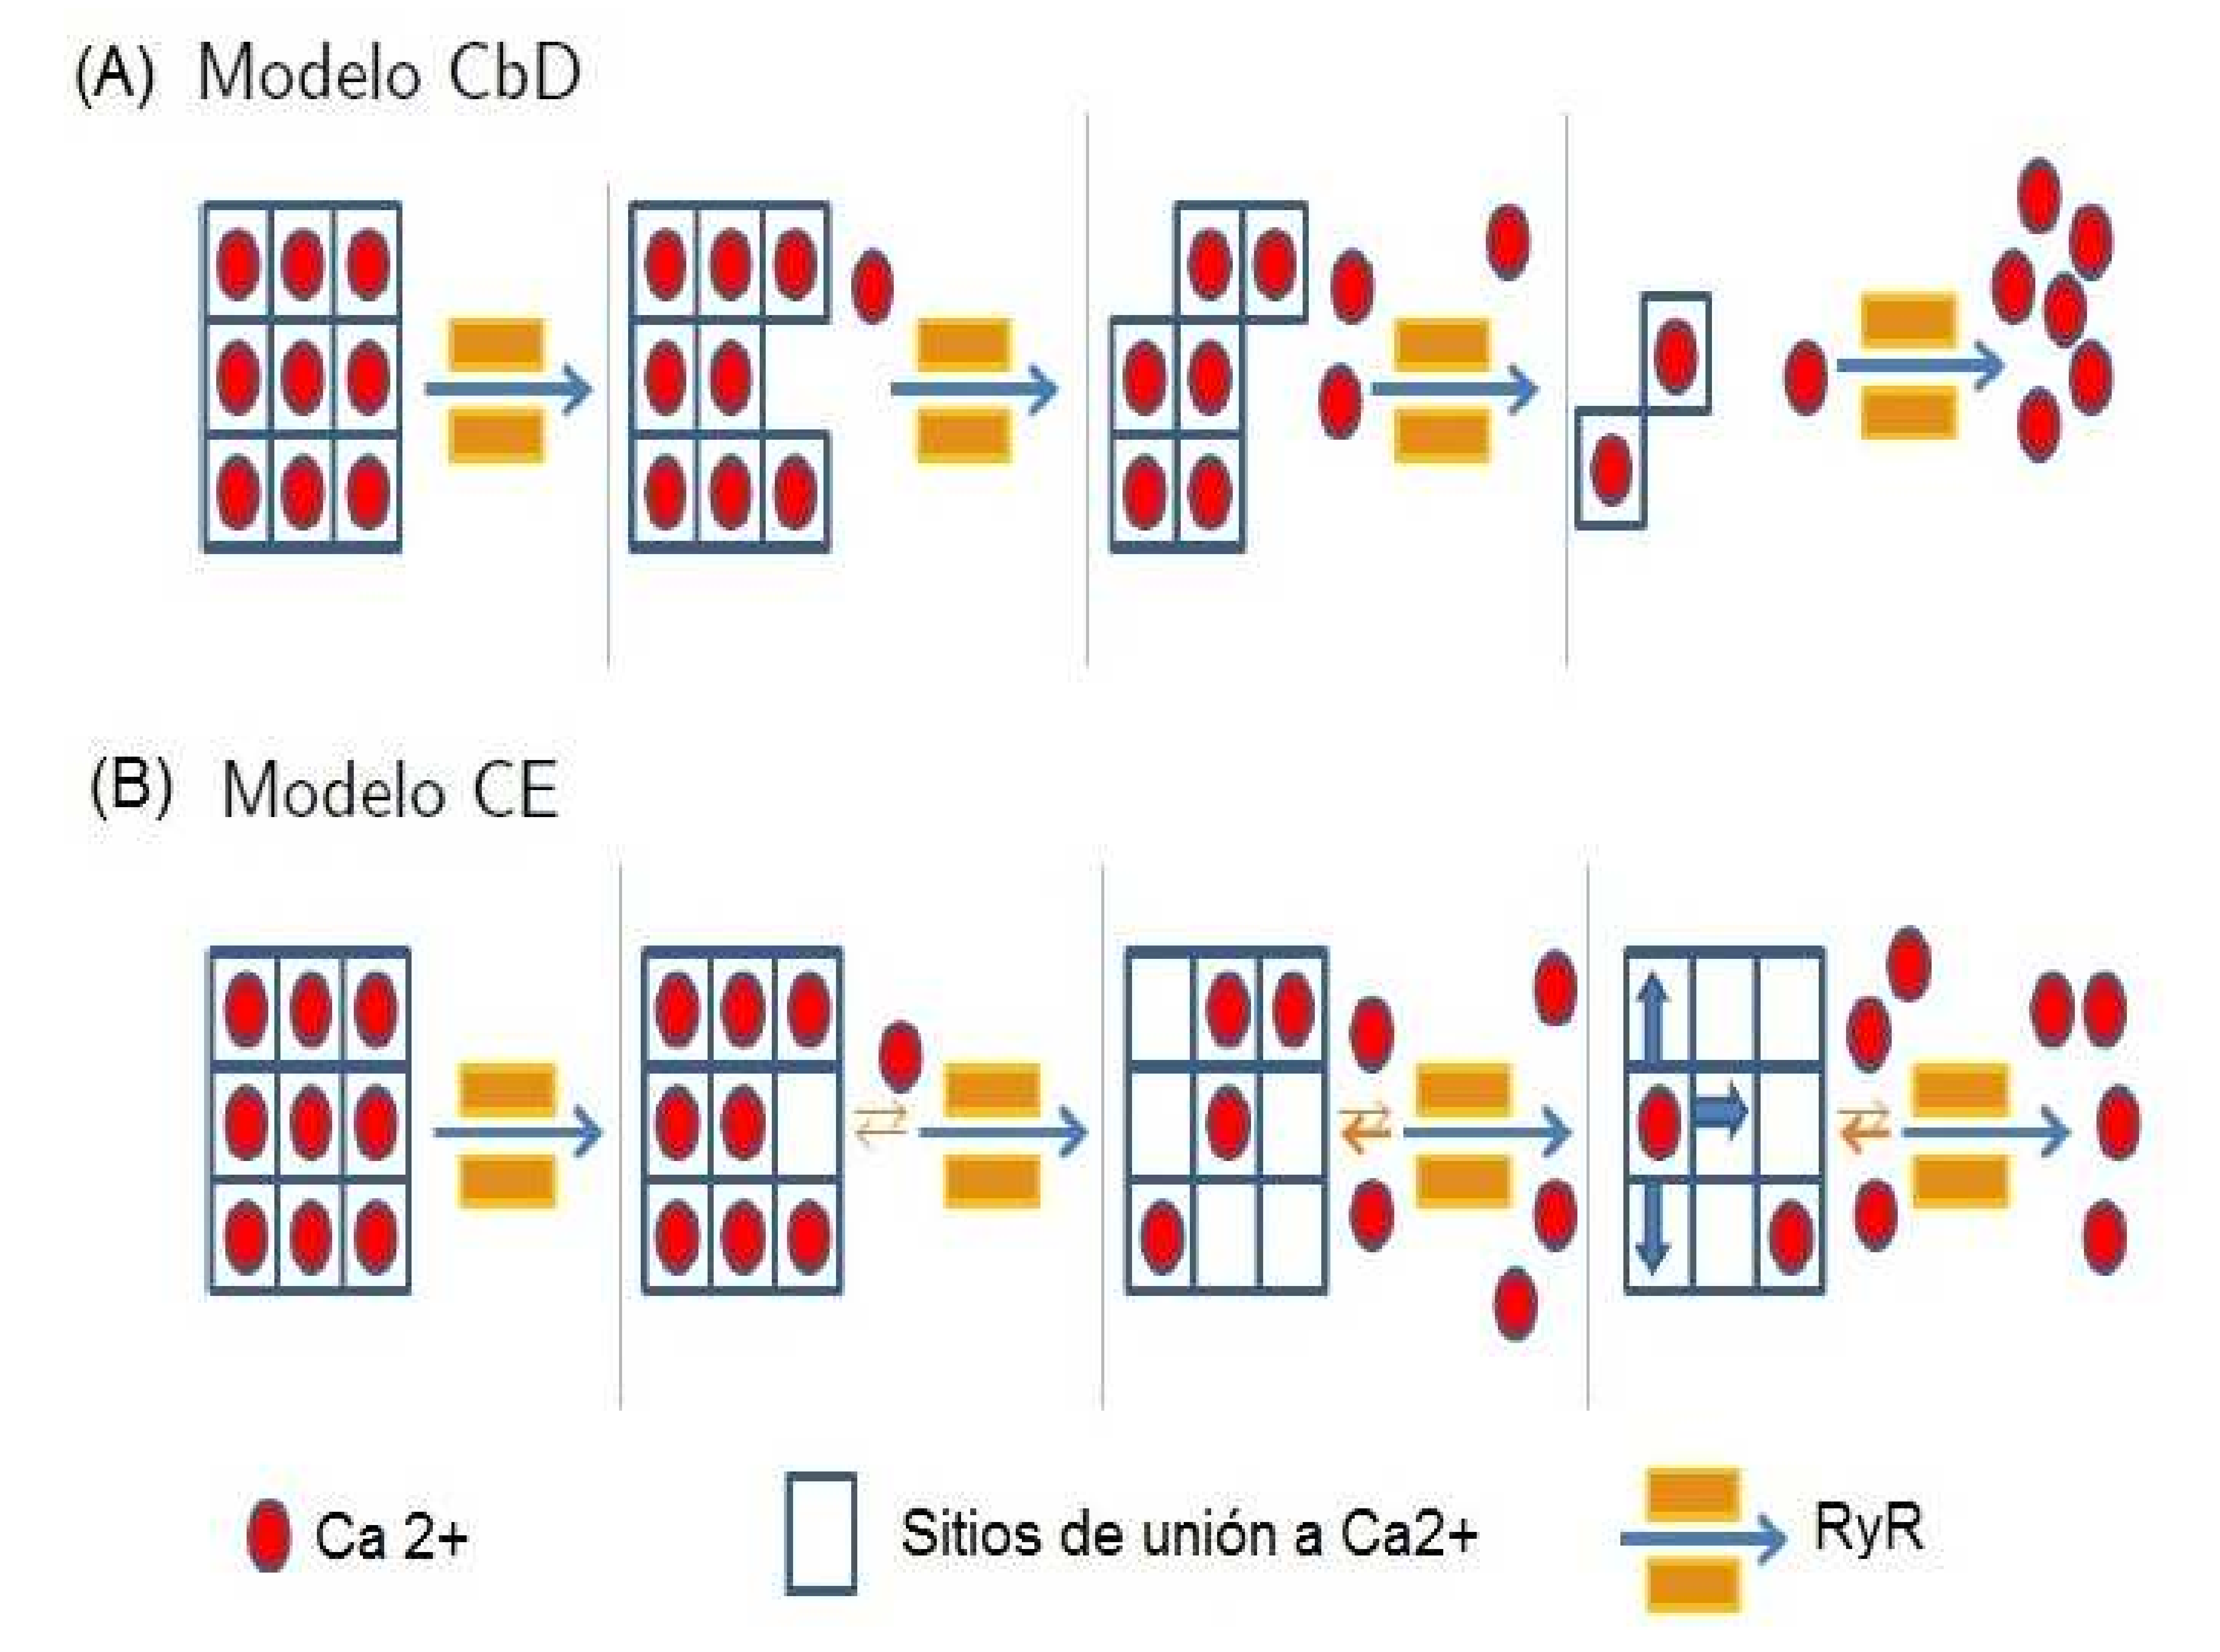
\includegraphics[width=.8\textwidth]{FIGURA12}
		\caption{{\tiny Norma Citlalcue Pérez Rosas. Análisis de la dinámica del ion calcio durante su liberación por
				medio de los receptores de rianodina : un enfoque de modelación matemática. Thesis, Centro de
				Investigación y de Estudios Avanzados del Instituto Politécnico Nacional, 2016.}}
	\end{figure}
	
\end{frame}

\begin{frame}{Antecedentes}
	
	\begin{figure}[h]
		\includegraphics[width=.8\textwidth]{FIGURA5}
		\caption{{\tiny Norma Citlalcue Pérez Rosas. Análisis de la dinámica del ion calcio durante su liberación por
				medio de los receptores de rianodina : un enfoque de modelación matemática. Thesis, Centro de
				Investigación y de Estudios Avanzados del Instituto Politécnico Nacional, 2016.}}
	\end{figure}
	
\end{frame}

\begin{frame}{Antecedentes}
	
	\begin{figure}[h]
		\includegraphics[width=.8\textwidth]{FIGURA6}
		\caption{{\tiny Norma Citlalcue Pérez Rosas. Análisis de la dinámica del ion calcio durante su liberación por
				medio de los receptores de rianodina : un enfoque de modelación matemática. Thesis, Centro de
				Investigación y de Estudios Avanzados del Instituto Politécnico Nacional, 2016.}}
	\end{figure}
	
\end{frame}

\begin{frame}{Antecedentes}
	
	\begin{figure}[h]
		\includegraphics[width=.8\textwidth]{FIGURA7}
		\caption{{\tiny Norma Citlalcue Pérez Rosas. Análisis de la dinámica del ion calcio durante su liberación por
				medio de los receptores de rianodina : un enfoque de modelación matemática. Thesis, Centro de
				Investigación y de Estudios Avanzados del Instituto Politécnico Nacional, 2016.}}
	\end{figure}
	
\end{frame}

\begin{frame}{Antecedentes}
	
	\begin{figure}[h]
		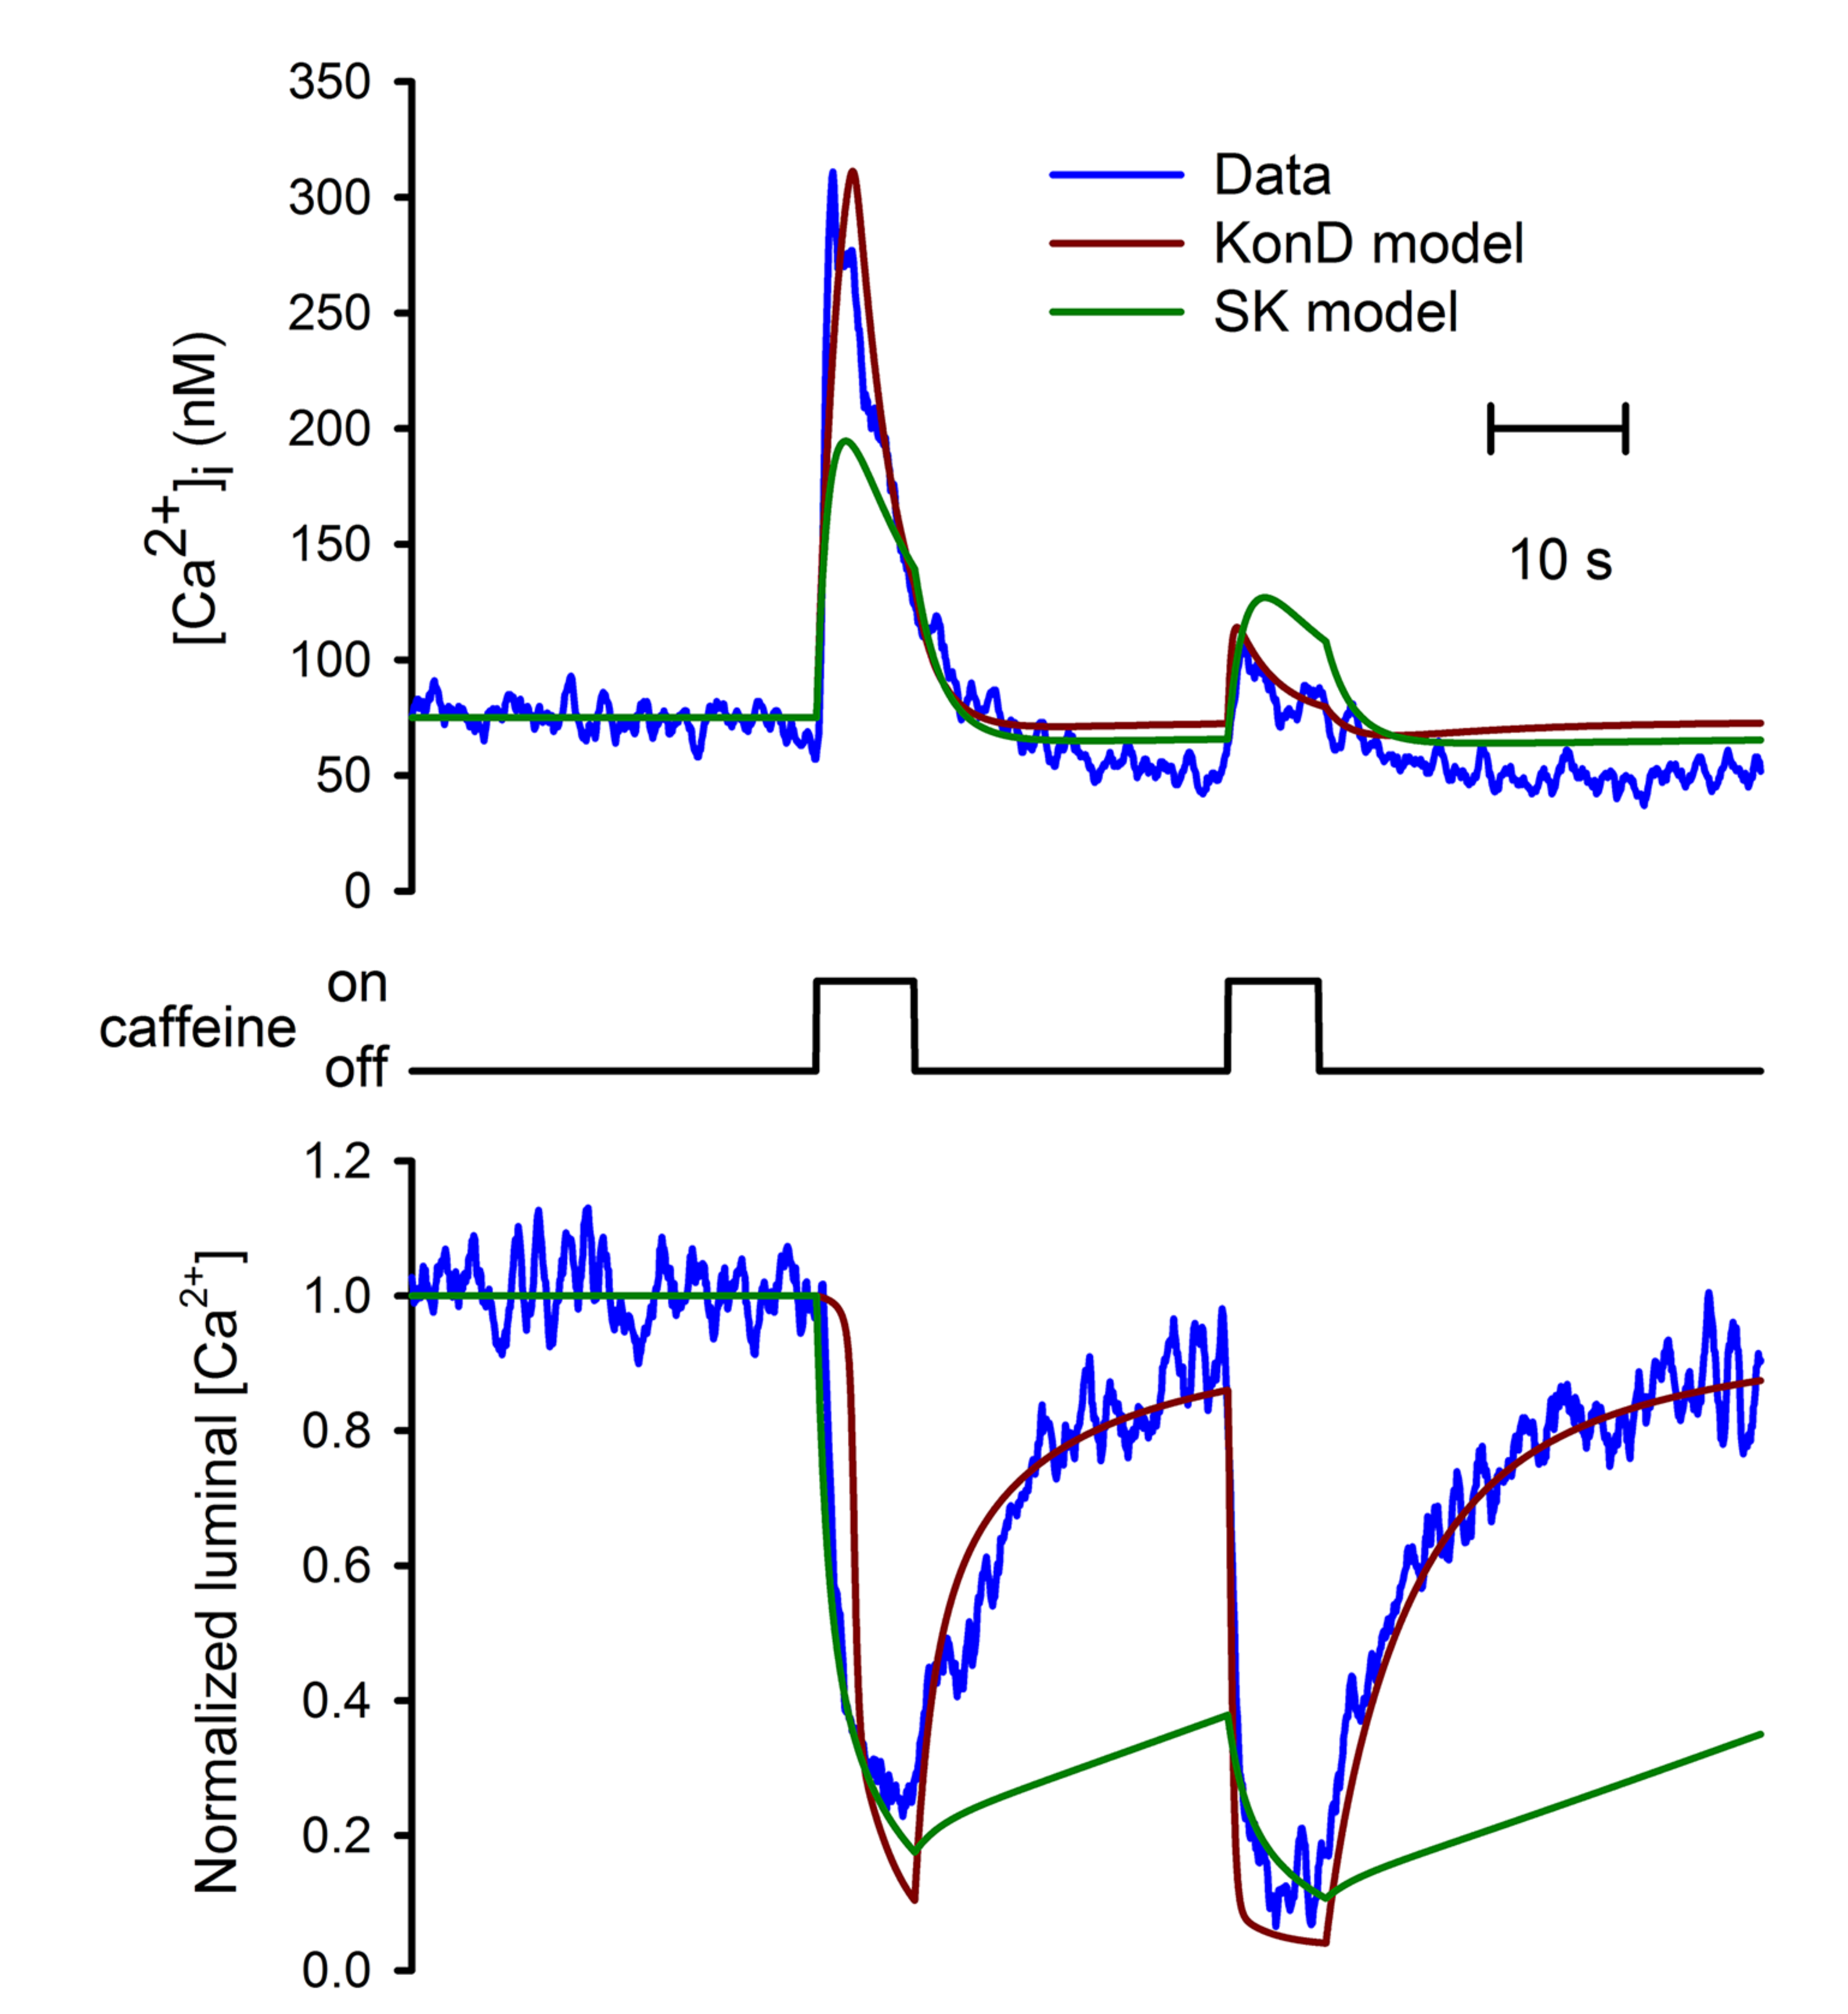
\includegraphics[width=.5\textwidth]{FIGURA8}
		\caption{{\tiny Norma Citlalcue Pérez Rosas. Análisis de la dinámica del ion calcio durante su liberación por
				medio de los receptores de rianodina : un enfoque de modelación matemática. Thesis, Centro de
				Investigación y de Estudios Avanzados del Instituto Politécnico Nacional, 2016.}}
	\end{figure}
	
\end{frame}